\chapter[Conversor]{Conversor Tensão frequência}

\section{Introdução}

\say{Conversores tensão-frequência(VFC) são osciladores de primeira ordem cuja a entrada é uma tensão analógica $V_{in}$ e tem como saída um sinal em frequência $f_0$ linearmente proporcional à tensão de entrada, portanto:
\begin{equation}
 f_0 = kV_{in}
 \label{eq01}
\end{equation}
 Eles geralmente são denominados conversores quase digitais devido à sua saída analógica traduzida em frequência.

Os VFCs geralmente são confundidos com osciladores controlados por tensão (VCOs), mas observe que os VFCs têm especificações de desempenho diferentes e mais rigorosas: os requisitos típicos são precisão de fator de alta escala e estabilidade com temperatura e tensão de alimentação, ampla faixa dinâmica e baixo erro de linearidade.} \cite{livroprincipal}

Há muitas abordagens para um VFC, na literatura a maioria se baseia no mesmo princípio de operação, que é a integração alternada da tensão de entrada que gera pulsos quando a tensão de saída se iguala à uma tensão de referência.
Os VFCs têm duas configurações principais, o multivibrador e o equilíbrio de carga. Suas diferenças podem ser vistas na atuação do circuito de controle: no multivibrador o circuito de controle impõe as tensões limite, ajustando a oscilação de tensão no capacitor, enquanto no equilíbrio de carga, o circuito de controle fixa a duração da fase de carga ou descarga.

O multivibrador é, geralmente, um conversor Corrente-Frequência(IFC) precedido pro um conversor Tensão-Corrente(VIC). Seu princípio de funcionamento e aplicação são bem simples e precisa de pouca potência, mas são menos precisos que o equilíbrio de carga.
O equilíbrio de carga pode ser síncrono ou assíncrono, ele é mais preciso que o multivibrador. Entretanto precisa de mais potência e o seu sinal de saída são trens de pulsos, diferente do multivibrador que é uma onda quadrada.
A escolha para o projeto da \textit{TAG} foi da abordagem do VFC multivibrador pela pouca potência necessária.

O diagrama na Fig. \ref{fig04} descreve o funcionamento do VFC projetado. Nele, uma tensão de entrada $V_{in}$ é aplicada num conversor tensão corrente, essa corrente é espelhada no circuito integrador bidirecional que manda o sinal de tensão para um circuito de controle que, realimenta o integrador com os comandos de carga e descarga do capacitor no integrador.

\begin{figure}[htb]
	\centering
	\includegraphics[width=0.9\textwidth]{figuras/blocks_diagram_vf.png}
	\caption{Diagrama de blocos VFC Multivibrador Fonte:\cite{livroprincipal} }
	\label{fig04}
\end{figure}



\begin{figure}[htb]
	\centering
	\includegraphics[width=0.6\textwidth]{figuras/sch_diagrama.png}
	\caption{Esquemático VFC Multivibrador Fonte:\cite{livroprincipal} }
	\label{fig05}
\end{figure}

\begin{figure}[htb]
	\centering
	\includegraphics[width=0.6\textwidth]{figuras/formas_ondas.png}
	\caption{Formas de onda do Capacitor e Saída do VFC Multivibrador Fonte:\cite{livroprincipal} }
	\label{fig06}
\end{figure}

Na Fig. \ref{fig05} há um exemplo implementado do modelo de VFC multivibrador funcional. Nele uma fonte de corrente controlada pela tensão de entrada $V_{in}$ gera uma corrente que é integrada num capacitor aterrado cuja as tensões variam entre duas referências, a tensão menor $V_L$ e a maior $V_H$. Ao observar a tensão no capacitor o circuito de controle atua no sentido de carga e descarga e também envia o sinal digital de saída com a frequência correspondente à tensão de entrada.  
A frequência de saída é obtida na onda exibida na Fig. \ref{fig06} onde o sinal digital acompanha as retas de subida e descida na tensão do capacitor do integrador. A sua expressão é dada na Eq. \ref{eq01}. 

\section{Conversor Tensão corrente} 

O conversor tensão corrente(VIC) é um bloco base para muitos designs de sinais analógicos e mistos como em multiplicadores, conversores de dados, amplificadores de ganho variável.O VIC é o estágio de entrada do VFC, a maior parte  da performance depende desse bloco. Isso leva à necessidade de uma transcondutância($gm$) independente de temperatura, tempo e tensão com variação linear e largura de banda apropriada.\cite{livroprincipal}.

A ideia descrita nos artigos \cite{artigo_principal} e \cite{artigo_tag_unb} em que o trabalho se baseia é que para a análise dos sinais vitais a tensão gerada pelos batimentos cardíacos é retificada e então é usada como a tensão de entrada $V_{in}$ do VFC. 

\begin{figure}[htb]
	\centering
	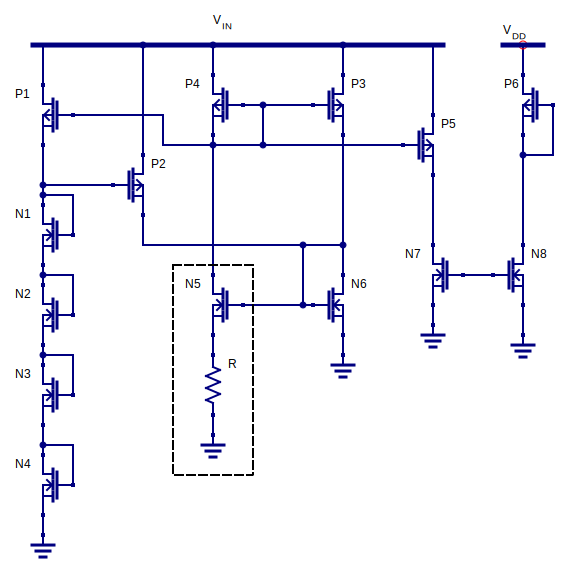
\includegraphics[width=0.8\textwidth]{figuras/v-i.png}
	\caption{Esquemático circuito conversor tensão corrente. Fonte:\cite{artigo_principal} }
	\label{fig07}
\end{figure}

A topologia do circuito VIC desse projeto está exibida na Fig. \ref{fig07}. Observa-se no esquemático uma variação de uma bootstrapped auto-bias current source, ou seja, fonte de correte auto enviesada. Nesse modelo a corrente, limitada pelo resistor, é espelhada de forma mútua entre os espelhos dos PMOS $P_3$ e $P_4$  e NMOS $N_5$ e $N_6$. 
A relação à esquerda, composta pelo divisor de tensão com $P_1$, $P_2$, $N_1$ até $N_4$, funciona como um soft-start que regula a corrente de acordo com a variação da tensão $V_{in}$ de forma proporcional às tensões do $P_2$. Essas razões de proporção estão expressas na eq. \ref{eq02}.

\begin{equation}
 V_{in}\propto V_{GS,P2}\propto V_{GS,N6} = V_{GS,N5} \Rightarrow V_{in}\propto V_{GS,N5} \approx \frac{1}{R}
 \label{eq02}
\end{equation}


\begin{table}[htb]
\centering
\begin{tabular}{c|c}
\hline 
\hline 
\textbf{Nome do componente} & \textbf{Dimensões (W/L)[$\mu$ m]} \\ 
\hline 
\hline 
$P_1$, $N_1$,$N_2$,$N_3$,$N_4$ & 1/5 \\ 
\hline 
$P_2$ & 0.24/0.18 \\ 
\hline 
$P_3$, $P_4$, $P_5$  & 0.24/21.82 \\ 
\hline 
$N_5$,$N_6$ & 15/45 \\ 
\hline 
$N_7$,$N_8$ & 0.24/20 \\ 
\hline 
$P_6$ & 100/2 \\ 
\hline 
$R$ & 200 $\Omega$ \\ 
\hline 
\end{tabular} 
\caption{Dimensões dos transistores e resistor do VIC}
\label{tab:vic}
\end{table}

 Á direita da fonte há um espelho, composto por $P_5$ e $N_7$, que direciona uma corrente que será espelhada novamente para uma relação, $P_6$ e $N_8$, cuja a tensão de alimentação não é mais a $V_{in}$, que é traduzida em corrente, mas sim a tensão $V_{DD}$ padrão de alimentação do resto do circuito. Essa tensão de saída é a tensão de Bias usada nos espelhos para o circuito integrador usado para criar o sinal de frequência.

Considerações devem ser feitas sobre esse circuito. O primeiro é sobre a faixa de corrente que ele vai abranger, que exerce influência direta nas frequências de saída. Além disso quanto maior essa faixa maior será a potência consumida. A potência máxima exigida no projeto pode afetar o desenvolvimento do projeto para se ajustar ao consumo total essas faixas podem ser revistas.

 O controle dessa faixa é feito com o dimensionamento dos transistores e depois do resistor. Sua linearidade é controlada com a relação W/L que deve ser pequena para evitar efeitos de canal curto. Entretanto isso afeta no ganho e na transcondutância tornando a faixa menor. O controle da transcondutância também é influenciado pelo resistor, que de acordo com o seu tamanho ele aumenta ou reduz a faixa de corrente. Portanto deve-se procurar um equilíbrio comum entre essas parâmetros para que um não se sobressaia e afete demais o outro.


\section{Integrador} 

O integrador bidirecional é um circuito de carga/descarga com um capacitor $C$ temporizado e uma fonte de corrente constante que carrega o capacitor e um dissipador constante que o descarrega. O controle da carga e descarga do capacitor é feito com um circuito que observa a tensão no capacitor e a compara com tensões de referência limites, alto($V_H$) e baixo($V_L$), e dá a ordem de carga ou descarga. O acionamento é feito com a ativação alternada das chaves que selecionam a carga ou descarga. 
O modelo explicativo em blocos está na Fig. \ref{fig08}.

\begin{figure}[htb]
	\centering
	\includegraphics[width=0.5\textwidth]{figuras/integrador_sch.png}
	\caption{Integrador de corrente bidirecional com fonte e espelho de corrente. Fonte:\cite{livroprincipal} }
	\label{fig08}
\end{figure}

Na Fig. \ref{fig09} está o circuito proposto. Para destrinchar o seu funcionamento ignore momentaneamente os transistores $P_2$ e $P_3$. O transistor $P_1$ espelha a corrente do circuito VIC apresentado anteriormente e atua como uma fonte de corrente para o integrador. 
Inicialmente o capacitor está descarregado, com isso o sistema de controle faz o integrador ligar o $P_5$ e a corrente é direcionada no capacitor carregando-o. 
A tensão no capacitor então aumenta com a injeção de corrente nele seguindo a expressão da eq. \ref{eq03}. Sendo $V_0$ a tensão inicial ou anterior à mudança de estado do capacitor.

\begin{equation}
V_{cap}(t) = V_0 + \frac{I\cdot t}{C_1}
 \label{eq03}
\end{equation}

Após a tensão $V_{cap}$ atingir o valor de $V_H$ ele troca os estados das chaves deligando $P_5$ e acionando $P_4$. 
Assim a corrente agora é direcionada para o lado esquerdo que espelha a corrente nos transistores $N_2$ e $N_4$ descarregando o capacitor até atingir $V_L$ e o sistema de controle alternar as chaves de novo.  


A frequência do processo da carga e descarga é obtido com a expressão da eq. \ref{eq04}, que já é a expressão da frequência final observada no VFC, apesar da tensão do capacitor $V_{cap}$ não ser o sinal de saída do VFC. 

\begin{equation}
f = \frac{I}{C\cdot(V_H - V_L)}
 \label{eq04}
\end{equation}

\begin{figure}[htb]
	\centering
%Erro cometido nesse esquemático
%Os inversores de P4 e P5 não são ligados no GND, mas sim no Vbias
	\includegraphics[width=0.7\textwidth]{figuras/integrate.png}
	\caption{Esquemático do Integrador de Corrente Bidirecional Fonte:\cite{artigo_tag_unb} }
	\label{fig09}
\end{figure}

Os transistores $N_1$ e $N_2$ estão ativados com uma tensão de bias o suficiente para ligá-los. Os $P_2$ e $P_3$ são acionados para atingir novas faixas de frequência. A ideia é de que ao acionar cada um dos transistores que espelha a corrente do VIC a faixa mude entre as opções: 100Hz-1kHz, 1kHz-10kHz e 10kHz-100kHz. Onde as correntes de $P_2$ e $P_3$  são somadas para alterar as frequências no integrador.

\begin{table}[htb]
\centering
\begin{tabular}{c|c}
\hline 
\hline 
\textbf{Nome do componente} & \textbf{Dimensões (W/L)[$\mu$ m]} \\ 
\hline 
\hline 
$P_6$, $P_7$, $N_5$ ,$N_6$ & 0.24/0.18 \\ 
\hline 
$P_4$, $P_5$, $N_1$,$N_2$,$N_3$,$N_4$ & 1/15 \\ 
\hline 
$P_8$, $P_9$, $P_10$  & 0.3/0.18 \\ 
\hline 
$P_1$ & 0.73/2 \\ 
\hline 
$P_2$ & 6.5/2 \\ 
\hline 
$P_3$ & 73/2 \\ 
\hline 
$C$ & 7pF \\ 
\hline 
\end{tabular} 
\caption{Dimensões dos transistores e capacitor do Integrador bidirecional}
\label{tab:integrador}
\end{table}


\section{Circuito de Controle} 

O circuito de controle usado é baseado na topologia da Fig. \ref{fig10}, onde são usado dois AmpOps como comparadores da tensão $V_{cap}$ com os limiares $V_H$ e $V_L$ e os seus sinais são usados na entrada de um latch SR. O latch recebe a saída da relação de AmpOps e, com os sinais $Q$ e $NQ$ realimenta esses sinais no circuito integrador. A saída final do VFC é o sinal $Q$ do circuito de controle.


\begin{figure}[htb]
     \centering
     \begin{subfigure}[b]{0.49\textwidth}
         \centering
         \includegraphics[width=\textwidth]{figuras/control_topology.png}
         \caption{Topologia do circuito de controle.}
         \label{fig10}
     \end{subfigure}
     \hfill
     \begin{subfigure}[b]{0.49\textwidth}
         \centering
         \includegraphics[width=\textwidth]{figuras/controle_waves.jpg}
         \caption{Formas de onda dos sinais esperados no sistema de controle}
         \label{fig11}
     \end{subfigure}
        \caption{Fonte:\cite{livroprincipal}}
        \label{fig:control}
\end{figure}

Em simulação o bloco do circuito foi feito como apresentado na Fig. \ref{fig12}, onde as tensões $V_H$ e $V_L$ são obtidas com os divisores de tensão dos transistores conectados em diodo.

\begin{figure}[htb]
	\centering
	\includegraphics[width=0.9\textwidth]{figuras/controle.png}
	\caption{Esquemático dos componentes do Circuito de controle acompanhados dos divisores de tensão para as tensões de Bias $V_H$ e $V_L$ Fonte:\cite{artigo_principal} }
	\label{fig12}
\end{figure}

\begin{table}[htb]
\centering
\begin{tabular}{c|c}
\hline 
\hline 
\textbf{Nome do componente} & \textbf{Dimensões (W/L)[$\mu$ m]} \\ 
\hline 
\hline 
$P_4$ & 1/2 \\ 
\hline 
$P_1$, $P_2$, $P_3$, $P_5$, $P_6$  & 1/5 \\ 
\hline 
\end{tabular} 
\caption{Dimensões dos transistores dos divisores de tensão para as tensões de Bias $V_H$ e $V_L$}
\label{tab:control}
\end{table}

\subsection{Latch SR}

O Latch SR pode ser descrito como um circuito digital primitivo de memória. Com ele é possível manusear estados e por tabela armazenar informação. Há dois tipos de Latch SR, o que se baseia em portas lógicas NOR e NAND.
O comportamento lógico desse circuito está descrito nas tabelas verdade das figuras \ref{fig13} e \ref{fig14}. Em resumo o do tipo NAND foi usado no projeto por conta do seu estado ser alterado para as condições desejadas no controlador com a queda nos sinais de SET($S$) e RESET($R$). Há abordagens que usa o Latch de tipo NOR, mas com inversores na entrada, isso é observado na Fig. \ref{fig10} por exemplo. 
O circuito do Latch SR montado a partir dos transistores MOS se encontra na Fig. \ref{fig15}. 

\begin{figure}[htb]
     \centering
     \begin{subfigure}[b]{0.49\textwidth}
         \centering
         \includegraphics[width=\textwidth]{figuras/lacthSR_NOR.png}
         \caption{Esquemático Latch SR tipo NOR}
         \label{fig13}
     \end{subfigure}
     \hfill
     \begin{subfigure}[b]{0.49\textwidth}
         \centering
         \includegraphics[width=\textwidth]{figuras/lachSR_NAND.png}
         \caption{Esquemático Latch SR tipo NAND}
         \label{fig14}
     \end{subfigure}
        \caption{Fonte:\cite{cmos_digital}}
        \label{fig:latch}
\end{figure}


\begin{figure}[htb]
	\centering
	\includegraphics[width=0.9\textwidth]{figuras/lach_sr_NAND.png}
	\caption{Topologia Latch SR do tipo NAND Fonte:\cite{cmos_digital} }
	\label{fig15}
\end{figure}

\begin{table}[htb]
\centering
\begin{tabular}{c|c}
\hline 
\hline 
\textbf{Nome do componente} & \textbf{Dimensões (W/L)[$\mu$ m]} \\ 
\hline 
\hline 
$P_1$, $P_2$, $P_3$, $P_4$, $N_1$, $N_2$, $N_3$, $N_4$  & 0.24/0.18 \\ 
\hline 
\end{tabular} 
\caption{Dimensões dos transistores do Latch SR NAND}
\label{tab:latch}
\end{table}

\subsection{Amplificador operacional}

Os comparadores do circuito de controle são AmpOps. Para o ampop foi usado a topologia de 2 estágios com cascode, como observado na Fig.\ref{fig16}. A tensão de Bias para polarização dos transistores $P_1$ e $P_6$ é feita com o espelho de corrente usando a fonte de tensão do projeto Cedro. As outras tensões de bias são obtidas com os divisores no canto inferior esquerdo. 

\begin{figure}[htb]
	\centering
	\includegraphics[width=0.9\textwidth]{figuras/ampop.png}
	\caption{ Fonte:\cite{cmos_analog} }
	\label{fig16}
\end{figure}

O ganho dessa topologia de AmpOp pode ser expresso pela eq. \ref{eq05} que quantifica a contribuição de ambos estágios no ganho final.


\begin{equation}
 A_V = g_{mP2}\cdot[(g_{mP5}r_{oP3}(r_{oP5})\parallel(g_{mN2}r_{oN2}(r_{oN4})]\cdot[(g_{mP7}r_{oP6}(r_{oP7})\parallel(g_{mN5}r_{oN5}(r_{oN6})]
 \label{eq05}
\end{equation}

\begin{table}[htb]
\centering
\begin{tabular}{c|c|c}
\hline 
\hline 
\textbf{Nome do componente} & \textbf{Dimensões (W/L)[$\mu$ m]} & Multiplier \\ 
\hline 
\hline 
$P_1$, $P_11$   & 0.4/0.2 & 1 \\  \hline
$P_6$   & 0.4/0.2 & 3 \\  \hline
$P_2$, $P_3$, $P_4$, $P_5$, $N_1$, $N_2$ & 0.3/0.18 & 1 \\  \hline
$N_3$, $N_4$ & 0.3/2.1 & 1 \\  \hline
$P_7$, $N_8$, $N_9$, $N_{11}$, $N_{12}$ & 0.24/0.18 & 1 \\  \hline
$N_{10}$ & 0.24/0.4 & 1 \\  \hline
$N_{14}$ & 0.24/0.18 & 1 \\  \hline
$N_{13}$ & 0.24/0.18 & 12 \\  \hline
$P_8$, $P_9$, $P_{10}$ & 1/5 & 1 \\  \hline
\end{tabular} 
\caption{Dimensões dos transistores do AmpOp de 2 estágios cascode}
\label{tab:ampop}
\end{table}


